\documentclass[journal,10pt,twocolumn]{IEEEtran}
\usepackage[T1]{fontenc}
\usepackage[utf8]{inputenc}
\usepackage{amsmath,amssymb,amsthm,mathtools}
\usepackage{graphicx,booktabs,array,algorithm,algorithmic,cite,url,microtype,tikz}
\usepackage[hidelinks]{hyperref}
\usetikzlibrary{arrows.meta,positioning}
\newtheorem{proposition}{Proposition}
\newtheorem{corollary}{Corollary}
\newcommand{\Fmax}{F_{\max}}
\newcommand{\EE}{\mathbb{E}}
\newcommand{\pmv}[2]{#1{\scriptsize$\pm$#2}}

\begin{document}
\title{Budget-Constrained Analyst Paging on Minute-Level IP Interaction Graphs: Online Rate Control, Verifier Gating and Incident-Level Evaluation}
\author{Asher Mehfooz%
\thanks{A.\ Mehfooz is with the University of Kotli Azad Jammu and Kashmir, Kotli, Pakistan (e-mail: asherzaki960@gmail.com; ORCID: 0009-0009-3570-9881).}}
\markboth{Manuscript under review}{Mehfooz: Budget-Constrained Analyst Paging}
\maketitle

\begin{abstract}
Security operations centres (SOCs) are limited less by detection accuracy than by how often a detector interrupts a human analyst. We treat the interrupt rate as a hard operational constraint, $F(\pi)\le\Fmax$, and study how detection, verification and budget control interact on streamed network data. Flows from CIC-IDS2017 and UNSW-NB15 are cut into 60-second IP interaction graphs and scored by degree statistics, Isolation Forest and small neural heads; an optional port-based verifier gates the scores; and three online controllers enforce the budget: a projected dual (Lagrangian) threshold, a hard running-rate mask, and a hybrid that adapts its threshold by the dual while the mask enforces the cap. We first show that the common CIC-IDS2017 flow export stores afternoon times on a 12-hour clock, which silently reorders each capture day, and we repair it and verify the repair against the published attack schedule. On both datasets, thresholds calibrated on training data exceed a 10\% budget by a factor of 1.8 to 2.8, and the plain Lagrangian controller exceeds it in 3 to 6 of 10 seeds. The hybrid never exceeds the budget in any seed, budget level or dataset, and reaches window true-positive rate $0.917\pm0.065$ on CIC-IDS2017 (with the verifier) and $0.818$ with full incident recall on UNSW-NB15 (without it). The port verifier helps on scan and flood traffic but hurts on UNSW-NB15's exploit-heavy mix, so the verifier must match the threat mix. We prove that the capped controllers page any alert preceded by $\lceil 1/\Fmax\rceil-1$ quiet windows, and we show that window-level TPR misjudges bursty attacks, so we report incident recall and time-to-page alongside it.
\end{abstract}

\begin{IEEEkeywords}
Alert fatigue, security operations, rate-constrained decisions, network intrusion detection, CIC-IDS2017, online control, graph features.
\end{IEEEkeywords}

\section{Introduction}
\IEEEPARstart{N}{etwork} intrusion detectors are usually evaluated by accuracy, true-positive rate (TPR) or the area under the ROC curve (AUROC) \cite{chandola2009anomaly,buczak2016survey,sharafaldin2018cicids}. Security operations centres are judged differently: by whether analysts can act on what they are sent. Field studies report that analysts receive far more alerts than they can investigate and that most are false positives \cite{alahmadi2022falsepos,kokulu2019soc}. Ranking and triage systems reduce this load \cite{hassan2019nodoze}, but they rarely state, let alone guarantee, how often a human will be interrupted.

This paper makes that quantity the constraint. Let $t$ index tumbling time windows and $a_t\in\{0,1\}$ indicate that the system pages an analyst after window $t$. The operator cost of a policy $\pi$ over $T$ windows is
\begin{equation}
F(\pi)=\EE_{\pi}\Bigl[\tfrac{1}{T}\textstyle\sum_{t=0}^{T-1}a_t\Bigr],
\label{eq:F}
\end{equation}
and the design goal is to detect as many attacks as possible subject to $F(\pi)\le\Fmax$. With $\Fmax=0.10$ and one-minute windows, at most six pages per hour reach the analyst. This is a constrained decision problem \cite{altman1999cmdp}; in the setting studied here the decision reduces to a time-varying threshold on a risk score, so we treat it as online rate-constrained thresholding \cite{cotter2019constraints,mahdavi2012longterm} rather than as a full constrained Markov decision process.

\subsection{Contributions}
\begin{enumerate}
\item \textbf{A data repair with measurable impact.} We show that the widely used CIC-IDS2017 flow export records afternoon timestamps on a 12-hour clock without an AM/PM marker, so a naive parse places every afternoon before its own morning. We give a one-line repair, verify it against the published attack schedule, and show that it changes every budget-relevant conclusion (Section~\ref{sec:clock}).
\item \textbf{A budgeted paging pipeline} that separates scoring (degree, Isolation Forest, neural heads on minute IP graphs), verification (a port-diversity verifier) and budget control (projected dual threshold, hard running-rate mask, or a hybrid of the two).
\item \textbf{A hybrid controller with guarantees.} The dual is driven by the \emph{requested} paging rate while the mask enforces the cap. We prove a pathwise budget, a quiet-period guarantee (an alert preceded by $\lceil1/\Fmax\rceil-1$ windows without a page is always paged) and a burst ceiling that explains why window-level TPR understates performance on bursty attacks (Section~\ref{sec:theory}).
\item \textbf{An evaluation built for SOCs on two datasets}: train-calibrated baselines, a controller-by-verifier ablation, a budget sweep from 2\% to 20\%, rolling-origin folds and incident-level metrics (incident recall, time-to-page, precision) on CIC-IDS2017 and UNSW-NB15.
\end{enumerate}

\subsection{Scope}
We do not deploy in a live SOC, do not train a language model, and do not claim optimality for neural scores. The verifier slot is designed to accept a language-model triage agent (Section~\ref{sec:llm}), but every number reported here uses the port-based verifier.

\section{Related Work}
\subsection{Flow and log detectors}
Flow classifiers on CIC-IDS2017 and UNSW-NB15 report flow-level accuracy \cite{sharafaldin2018cicids,moustafa2015unsw,ring2019unsw}. Log-based detectors such as DeepLog treat a host as a token stream \cite{du2017deeplog,he2017drain,xu2009lsa}. Sommer and Paxson \cite{sommer2010closed} and Arp \emph{et al.} \cite{arp2022dos} warn that such evaluations often ignore operational cost, temporal ordering and base rates. Engelen \emph{et al.} \cite{engelen2021troubleshooting} and Lanvin \emph{et al.} \cite{lanvin2023errors} documented labelling and feature-extraction errors in CIC-IDS2017. The timestamp issue we report is, to our knowledge, not among them, and it matters specifically for time-ordered evaluation.

\subsection{Graphs for intrusion detection}
Provenance systems reconstruct attack stories from audit graphs \cite{king2003backtracking,hossain2017sleuth,milajerdi2019holmes,cheng2024kairos,rehman2024flash}. Network-level graph detectors embed flow graphs with graph neural networks \cite{lo2022egraphsage,hamilton2017graphsage,kipf2017gcn} or predict temporal links for lateral movement \cite{king2022euler}. Temporal graph networks maintain node memories on timestamped edges \cite{rossi2020tgn,kumar2019jodie,pareja2020evolvegcn}, and graph anomaly surveys cover density and residual scores \cite{akoglu2015graph}. These works optimise detection quality; none bounds the rate at which a human is interrupted. Our window encoder is deliberately simple (aggregate graph statistics with an exponential moving average) so that the effect of budget control can be isolated; any of these encoders can replace it.

\subsection{Alert volume and triage}
NoDoze ranks provenance alerts by anomaly propagation \cite{hassan2019nodoze}, and SOC studies document alert fatigue directly \cite{alahmadi2022falsepos,kokulu2019soc}. Ranking orders alerts but does not cap their number.

\subsection{Budgeted and selective decisions}
Rate-constrained classification optimises accuracy subject to a positive-prediction rate \cite{cotter2019constraints}; online convex optimisation with long-term constraints bounds cumulative violation \cite{mahdavi2012longterm}; selective classification and learning to defer decide when to hand a case to a human \cite{geifman2017selective,mozannar2020defer}; conformal risk control bounds expected loss under exchangeability \cite{angelopoulos2024crc}. Constrained policy optimisation solves constrained MDPs in control tasks \cite{achiam2017cpo,tessler2019rcpo,altman1999cmdp}. The SOC paging problem combines a hard rate constraint with strongly non-exchangeable, bursty data, which is why we study both a dual controller and a pathwise mask.

\subsection{Language models in security operations}
Instruction-tuned models summarise logs and alerts \cite{liu2023logprompt,motlagh2024llmsec}, and parameter-efficient tuning makes 7-8B models trainable locally \cite{hu2022lora,dettmers2023qlora,dubey2024llama3}. Running a language model on every flow is not a streaming algorithm; placing it behind a cheap score and a budget is the design question this paper's verifier slot addresses.

\section{Data and Clock Repair}
\label{sec:clock}
\subsection{Sources}
CIC-IDS2017 \cite{sharafaldin2018cicids}: the flow export \texttt{Network-Flows/CICIDS\_Flow.parquet} in the Hugging Face repository \texttt{rdpahalavan/CIC-IDS2017} (2\,827\,677 flows with source and destination IP, destination port, timestamp and label; SHA-256 \texttt{e64f6adf\ldots0dda35}). UNSW-NB15 \cite{moustafa2015unsw}: \texttt{Network-Flows/UNSW\_Flow.parquet} in \texttt{rdpahalavan/UNSW-NB15} (2\,059\,415 raw flows with IP addresses, Unix start time and attack category). Unlike the widely used training/testing partitions of UNSW-NB15, the raw flows keep addresses and time, so IP graphs can be built.

\subsection{The 12-hour clock}
After parsing, the flows fall into ten blocks of about four hours, separated by gaps that alternate between about 234 and 720 minutes. CIC-IDS2017 was captured from about 09:00 to 17:00 on five weekdays. The pattern matches exactly what happens when afternoon times are written as \texttt{1:00} to \texttt{5:00} without an AM/PM marker: each afternoon is parsed as 01:00 to 05:00 and is placed four hours \emph{before} its own morning. The consequences for any time-ordered study are severe: the ``past'' of a morning window contains the same day's afternoon, exponential moving averages run backwards across noon, and a 70/30 split cuts the data at the wrong place. The raw timestamps confirm the diagnosis: hours take only the values 1 to 5 and 8 to 12, and no flow carries an hour from 13 to 17. Because the capture contains no traffic between 01:00 and 07:59, the repair is unambiguous: add 12 hours to any timestamp whose hour lies in $[1,7]$. After repair the data form five contiguous blocks, one per weekday (Table~\ref{tab:data}), and the attack labels fall exactly on the published schedule \cite{sharafaldin2018cicids}: for example FTP-Patator begins at 09:17 and SSH-Patator at 14:09 on Tuesday, DoS Hulk runs 10:43 to 11:07 on Wednesday, and DDoS runs 15:56 to 16:16 on Friday. Without the repair, SSH-Patator and DDoS would appear to start at 02:09 and 03:56.

\subsection{Windows, graphs and labels}
Window $t$ holds the flows whose repaired timestamp falls in minute $t$. The nodes of $G_t=(V_t,E_t)$ are the source and destination IPs, and each flow is a directed edge. A window is labelled positive ($y_t=1$) when at least half of its flows carry a non-benign label (an \emph{attack-dominant minute}). Under the alternative ``any malicious flow'' rule, 21\% of minutes are positive and mostly-benign minutes dominate the positive class; the 50\% rule instead asks whether this minute should open an incident. An \emph{incident} is a maximal run of consecutive positive windows.

\begin{table}[t]
\centering
\caption{CIC-IDS2017 minute windows after clock repair.}
\label{tab:data}
\setlength{\tabcolsep}{4pt}
\footnotesize
\begin{tabular*}{\columnwidth}{@{\extracolsep{\fill}}lccccc@{}}
\toprule
 & Mon & Tue & Wed & Thu & Fri \\
\midrule
Windows & 486 & 488 & 509 & 486 & 484 \\
Positive windows & 0 & 0 & 24 & 0 & 30 \\
\midrule
\multicolumn{6}{@{}l}{Flows 2\,827\,677; non-benign 556\,555 (19.7\%)}\\
\multicolumn{6}{@{}l}{Mean edges per window: 1153}\\
\multicolumn{6}{@{}l}{Train / test windows: 1717 / 736 (split in Thursday)}\\
\multicolumn{6}{@{}l}{Positives by attack: DDoS 20, DoS Hulk 18, PortScan 10,}\\
\multicolumn{6}{@{}l}{\quad DoS GoldenEye 5, DoS Slowhttptest 1}\\
\multicolumn{6}{@{}l}{Train incidents (lengths, min): 1, 18, 1, 2, 2}\\
\multicolumn{6}{@{}l}{Test incidents (lengths, min): 6, 2, 2, 20 (all Friday)}\\
\bottomrule
\end{tabular*}
\end{table}

Table~\ref{tab:data} exposes three properties that any honest evaluation on this data must state. First, attack-dominant minutes occur on only two days and are all volumetric (DDoS, DoS, PortScan): Tuesday's brute-force and Thursday's web and infiltration attacks never dominate a minute. Second, the test split contains only 30 positive windows in four incidents, so window TPR moves in steps of $0.033$ and incident recall in steps of $0.25$. Third, positives are bursty: one test incident lasts 20 minutes.

\subsection{UNSW-NB15 windows}
UNSW-NB15 yields 1441 minute windows in two capture blocks (743 and 698 minutes). Its attacks are diffuse: 4.8\% of flows are malicious, they occur in 56\% of minutes, and no minute is attack-dominant. We therefore label a UNSW-NB15 window positive when at least 20\% of its flows are malicious (an \emph{elevated-attack minute}; 21 positives, prevalence 1.5\%, close to CIC-IDS2017's 2.2\%) and report a 10\% threshold as a sensitivity check. The 70/30 time split gives 1008 training windows (10 positives, three incidents) and 433 test windows (11 positives, four incidents of two to three minutes).

\section{Method}
\begin{figure}[t]
\centering
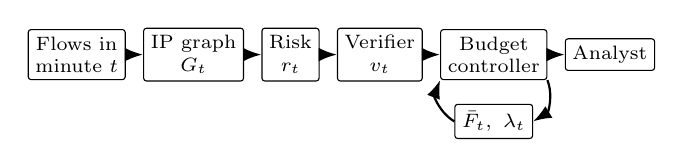
\begin{tikzpicture}[font=\scriptsize,box/.style={draw,rounded corners=1pt,inner sep=2.6pt,align=center},arr/.style={-{Latex},thick}]
\node[box] (a) {Flows in\\minute $t$};
\node[box,right=0.22cm of a] (b) {IP graph\\$G_t$};
\node[box,right=0.22cm of b] (c) {Risk\\$r_t$};
\node[box,right=0.22cm of c] (d) {Verifier\\$v_t$};
\node[box,right=0.22cm of d] (e) {Budget\\controller};
\node[box,right=0.22cm of e] (f) {Analyst};
\node[box,below=0.3cm of e] (g) {$\bar F_t,\ \lambda_t$};
\draw[arr] (a)--(b); \draw[arr] (b)--(c); \draw[arr] (c)--(d); \draw[arr] (d)--(e); \draw[arr] (e)--(f);
\draw[arr] (e.south east) to[bend left=40] (g.east); \draw[arr] (g.west) to[bend left=40] (e.south west);
\end{tikzpicture}
\caption{Pipeline. Tier 1 scores each minute graph; the verifier gates the score; the controller pages only if its running state ($\bar F_t$, and $\lambda_t$ for the dual) allows it.}
\label{fig:arch}
\end{figure}

\subsection{Tier 1: window scores}
Let $n_t=|E_t|$ and let $d^{\mathrm{out}}_{\max,t}$ be the largest out-degree in $G_t$. The only state carried between windows is $u_t=\alpha u_{t-1}+(1-\alpha)d^{\mathrm{out}}_{\max,t}$ with $\alpha=0.7$. The \emph{structure} vector contains the logarithms of $1+n_t$, of the numbers of distinct sources and destinations, of $1+d^{\mathrm{out}}_{\max,t}$, of the median flow duration, of the mean forward packet count and of $1+u_t$, together with the fraction of edges between distinct hosts. The \emph{full} vector adds destination-port diversity and the fraction of destination ports $\ge 10^4$. Features are standardised with training statistics.

We compare four scorers: (i) \emph{degree}, $r_t=\min(1,d^{\mathrm{out}}_{\max,t}/q_{0.7})$ with $q_{0.7}$ the training 70th percentile; (ii) Isolation Forest \cite{liu2008iforest} on the full vector, rescaled with training-score percentiles only; (iii) a structure MLP and (iv) a full MLP (two hidden layers of 32 and 16 units, class-weighted binary cross-entropy, 40 epochs of Adam).

\subsection{Verifier}
The verifier is a port heuristic computed with training quantiles,
\begin{equation}
v_t=\mathbf{1}\{\text{ports}_t\ge q_{0.75}\}\ \vee\ \mathbf{1}\{\text{high-port}_t\ge q_{0.70}\}.
\end{equation}
It flags minutes with unusual port diversity, the signature of scans and many denial-of-service tools. On its own it is a high-recall, high-volume detector; its role is to veto neural alarms that lack port evidence.

\subsection{Tier 2: budget controllers}
Each controller sees the stream once, in time order, and decides $a_t$ before window $t+1$ arrives. Let $h_t=\mathbf{1}\{r_t\ge\theta_t\}$ (\emph{hot}), optionally multiplied by $v_t$, and let $N_t=\sum_{s<t}a_s$.

\emph{Train-calibrated threshold.} $\theta$ is fixed at the $(1-\Fmax)$ quantile of the training scores. It meets the budget only if the score distribution does not shift.

\emph{Projected dual (Lagrangian).} $\theta_t=\theta_0+\kappa\lambda_t$ and
\begin{equation}
\lambda_{t+1}=\Pi_{[0,\lambda_{\max}]}\bigl(\lambda_t+\eta\,(N_{t+1}/(t+1)-\Fmax)\bigr),
\end{equation}
with $\theta_0=0.5$, $\kappa=0.08$, $\eta=0.25$, $\lambda_{\max}=8$. This is the standard dual update for a long-term rate constraint \cite{mahdavi2012longterm,tessler2019rcpo}; it targets the constraint on average and offers no pathwise guarantee.

\emph{Hard mask.} With fixed $\theta_0=0.5$, page iff
\begin{equation}
h_t=1\quad\text{and}\quad N_t+1\le\Fmax\,(t+1).
\label{eq:mask}
\end{equation}

\emph{Hybrid.} The threshold follows the dual, $\theta_t=\theta_0+\kappa\lambda_t$, and the page is accepted only under the mask condition \eqref{eq:mask}. Because the mask keeps the realised rate below $\Fmax$, a dual driven by realised pages would never rise; the hybrid therefore drives it by the \emph{requested} rate $W_{t+1}/(t+1)$, where $W_t=\sum_{s<t}h_s$ counts hot windows whether or not they were paged. The threshold thus rises whenever demand exceeds the budget, which preserves slack for the highest-scoring windows.

\emph{Rising-edge paging.} Optionally, a controller pages only when $h_t=1$ and $h_{t-1}=0$, so a sustained alarm produces one page per alert episode.

\begin{algorithm}[t]
\caption{Budgeted paging over a window stream}
\label{alg:pipe}
\begin{algorithmic}[1]
\STATE fit scorers and verifier quantiles on training windows
\STATE $N\leftarrow 0$, $\lambda\leftarrow 0$, $h_{\mathrm{prev}}\leftarrow 0$
\FOR{test window $t=0,1,\dots$}
\STATE $h\leftarrow\mathbf{1}\{r_t\ge\theta_t\}\cdot v_t$ \hfill(dual: $\theta_t=\theta_0+\kappa\lambda$)
\STATE $w\leftarrow h\wedge\neg(\text{edge}\wedge h_{\mathrm{prev}})$; $h_{\mathrm{prev}}\leftarrow h$
\STATE mask, hybrid: $a_t\leftarrow w\wedge(N+1\le\Fmax(t+1))$; dual: $a_t\leftarrow w$
\STATE $N\leftarrow N+a_t$; $W\leftarrow W+w$
\STATE dual: $\lambda\leftarrow\Pi(\lambda+\eta(N/(t+1)-\Fmax))$; hybrid: same with $W$ for $N$
\ENDFOR
\end{algorithmic}
\end{algorithm}

\section{Properties of the Capped Controllers}
\label{sec:theory}
All statements hold for every realisation of the stream, with no assumption on the score or the data. They use only the acceptance rule \eqref{eq:mask} and hold for any sequence of hot indicators $h_t$, including one produced by a time-varying threshold; they therefore apply to both the hard mask and the hybrid.

\begin{proposition}[Pathwise budget]
Under \eqref{eq:mask}, $N_t\le\Fmax\,t$ for all $t\ge 0$.
\end{proposition}
\begin{proof}
$N_0=0$. If $a_t=1$ then $N_{t+1}=N_t+1\le\Fmax(t+1)$ by \eqref{eq:mask}; if $a_t=0$ then $N_{t+1}=N_t\le\Fmax t\le\Fmax(t+1)$.
\end{proof}

\begin{proposition}[Quiet-period guarantee]
If no page was issued in the $m$ windows preceding $t$ and $m\ge\lceil1/\Fmax\rceil-1$, then a hot window $t$ is paged.
\end{proposition}
\begin{proof}
No page in $[t-m,t)$ gives $N_t=N_{t-m}\le\Fmax(t-m)$ by Proposition~1. Hence $N_t+1\le\Fmax(t-m)+1\le\Fmax(t+1)$ whenever $\Fmax(m+1)\ge1$, which holds for $m\ge\lceil1/\Fmax\rceil-1$.
\end{proof}

\begin{proposition}[Burst ceiling]
Let $s_t=\Fmax\,t-N_t\ge0$ be the accrued slack. In any $L$ consecutive windows starting at $t$, the mask issues at most $s_t+\Fmax L$ pages.
\end{proposition}
\begin{proof}
By Proposition~1, $N_{t+L}-N_t\le\Fmax(t+L)-N_t=s_t+\Fmax L$.
\end{proof}

\begin{corollary}
For an incident of length $L$ whose windows are all hot, the window TPR of the mask on that incident is at most $(s_t+\Fmax L)/L$, while its incident recall is $1$ whenever the incident is preceded by $\lceil1/\Fmax\rceil-1$ quiet windows.
\end{corollary}

With $\Fmax=0.10$, nine quiet minutes guarantee the next alarm is paged, and a 20-minute flood with no stored slack yields at most two pages, a window TPR of $0.10$ for an incident that was in fact caught at once. Window TPR therefore penalises the mask for declining to page an analyst who is already handling the incident. Two further consequences follow. False pages consume slack, so a permissive fixed threshold (low $\theta_0$, no verifier) starves later incidents; the hybrid counters this by raising its threshold when demand exceeds the budget. And the uncapped dual controller has none of these guarantees: $\lambda_t$ reacts only after the running rate exceeds $\Fmax$, so overshoot is expected when the score distribution shifts upward.

\section{Experimental Setup}
On CIC-IDS2017 the 2453 windows are split in time order: the first 70\% (Monday to mid-Thursday, 1717 windows) for fitting and the remaining 736 for testing; UNSW-NB15 is split the same way (Section~\ref{sec:clock}). Ten seeds vary MLP initialisation and Isolation Forest randomisation; we report mean $\pm$ sample standard deviation, and the number of seeds in which the realised interrupt rate exceeds $\Fmax$. To separate data uncertainty from seed noise we also use rolling-origin folds (train on all earlier days, test on Thursday or on Friday) and a moving-block bootstrap (block length 30) over test windows. Metrics: window TPR, false-alarm rate (FAR), interrupt rate, precision, incident recall (fraction of incidents with at least one page) and time-to-page (minutes from incident start to its first page, over detected incidents). $\Fmax=0.10$ is fixed in advance as an analyst-load assumption (one page per window, six minutes per hour); Section~\ref{sec:sweep} varies it from 0.02 to 0.20. Experiments run on a CPU; scoring the full test stream takes well under a second.

\section{Results}
\subsection{Effect of the clock repair}
Under the naive parse, the structure MLP appeared to meet the 10\% budget unaided (interrupt $0.098$), the Lagrangian controller met it on average ($0.095$), and degree paging used $0.278$ of minutes. Under the repaired clock the same configurations use $0.158$, $0.116$ (violating the budget in 6 of 10 seeds) and $0.346$. The repair changes both which policies are feasible and which policy is best, and it is the prerequisite for every result below.

\begin{table*}[t]
\centering
\caption{Test results at $\Fmax=0.10$ on CIC-IDS2017 after clock repair (736 windows, 30 positive windows, 4 incidents; 10 seeds, mean $\pm$ s.d.). ``Over'' counts seeds whose interrupt rate exceeds $\Fmax$. Incident recall is out of 4 incidents.}
\label{tab:main}
\setlength{\tabcolsep}{5pt}
\footnotesize
\begin{tabular}{@{}llcccccc@{}}
\toprule
Group & Policy & Window TPR & FAR & Interrupt & Precision & Incident recall & Over \\
\midrule
\csname @@input\endcsname tab_main_rows.tex
\bottomrule
\end{tabular}
\end{table*}

\subsection{Main comparison on CIC-IDS2017}
Table~\ref{tab:main} lists all policies at $\Fmax=0.10$. Scoring quality is high: AUROC is $0.987\pm0.024$ for the structure MLP, $0.976\pm0.009$ for Isolation Forest, $0.971\pm0.024$ for the full MLP and $0.841$ for degree. Ranking quality does not translate into budget compliance, however. Every unconstrained scorer and both train-calibrated thresholds exceed the budget in almost every seed; the calibrated thresholds page on $18\%$ of test minutes, 1.8 times the budget, because the test period (Thursday afternoon and Friday) is busier than the training period. A threshold fitted offline therefore cannot hold a budget under drift, which is the basic argument for online control.

Online control alone is not enough. The plain Lagrangian controller still exceeds the budget in 6 of 10 seeds, because $\lambda_t$ starts at zero and rises only after the rate is already too high. The plain hard mask stays within budget by construction but reaches window TPR of only $0.380$ and incident recall of $0.675$: false pages consume the slack that later incidents need (Proposition~3).

The verifier changes every controller on this dataset. Gating the full MLP with the verifier nearly halves the FAR (from about $0.083$ to $0.046$) and raises precision to about $0.46$ to $0.51$. With it the Lagrangian controller reaches TPR $0.927$ at interrupt $0.082$ (one seed over budget), the hard mask $0.837$ at $0.079$, and the hybrid $0.917$ at $0.075$ with the highest precision of any policy ($0.512$) and no seed over budget. The hybrid thus matches the recall of the dual while keeping the guarantees of the mask. Neither the verifier nor the controller is sufficient alone: the verifier with no controller pages on $36\%$ of minutes.

\subsection{Controller-by-verifier ablation}
The original version of this study reported a hard-mask TPR of $0.377$ and attributed it to the mask itself. The ablation in Table~\ref{tab:main} shows that the cause was the prefilter: the same masked policy at $\theta_0=0.35$ reaches TPR $0.367$, but at $\theta_0=0.5$ it reaches $0.837$, with identical guarantees. A permissive prefilter turns the mask into a first-come, first-served queue for false alarms, which is precisely what the hybrid's adaptive threshold prevents. A moving-block bootstrap over test windows for a single seed puts the TPR difference between the two prefilters in $[-0.55,0.85]$ (95\%): with four test incidents the data-level uncertainty is large even though the effect is consistent across all ten seeds.

\subsection{Incident-level view}
Every controlled policy that detects an incident does so within its first minute on average (mean time-to-page $0.12$ minutes for the verifier-gated controllers). Incident recall (about $0.83$) is the operational figure: of the four Friday incidents, three to four are paged per seed. Rising-edge paging is a different operating point. It pages once per alert episode, uses only $3.8\%$ of minutes, and still reaches incident recall $0.725$; its window TPR of $0.097$ is low by design and illustrates how misleading window TPR is for bursty attacks (Corollary~1).

\subsection{Budget sweep}
\label{sec:sweep}
\begin{figure*}[t]
\centering
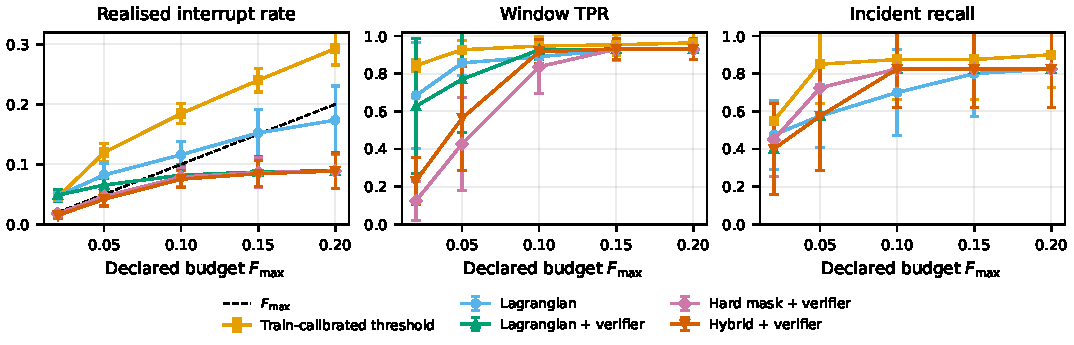
\includegraphics[width=\textwidth]{figs/fig_sweep.pdf}
\caption{Budget sweep on CIC-IDS2017 (10 seeds, mean $\pm$ s.d.). Left: realised interrupt rate against the declared budget (dashed line: equality). Middle: window TPR. Right: incident recall (4 test incidents).}
\label{fig:sweep}
\end{figure*}
Figure~\ref{fig:sweep} varies $\Fmax$ from $0.02$ to $0.20$. The capped controllers (mask and hybrid) never exceed the budget at any level in any seed. The Lagrangian controllers fail at tight budgets: at $\Fmax=0.02$ the realised rate is $0.047$ to $0.049$ (all seeds over), and at $\Fmax=0.05$ the verifier-gated variant is over in 9 of 10 seeds. The cause is the controller's lag: $\lambda_t$ needs many windows of excess paging before $\theta_t$ rises far enough. The hybrid dominates the mask at tight budgets (TPR $0.563$ against $0.427$ at $\Fmax=0.05$) because it raises its threshold instead of spending slack on the first hot windows. At loose budgets ($\Fmax\ge0.15$) the verifier-gated controllers no longer use their full allowance (interrupt about $0.09$), because the verifier rather than the budget becomes the binding filter, and TPR saturates at $0.93$. The train-calibrated threshold overshoots by a factor of 1.5 to 2.3 at every budget.

\subsection{Rolling-origin day folds}
Training on Monday to Wednesday and testing on Thursday (no attack-dominant minutes) measures pure false-alarm load: the verifier-gated Lagrangian, mask and hybrid page on $4.4\%$ to $4.5\%$ of minutes with no budget violation, whereas the plain Lagrangian ($9.1\%$) and the calibrated threshold ($9.8\%$) exceed the budget in 6 of 10 seeds. Training on Monday to Thursday and testing on Friday reproduces the main ranking: verifier-gated Lagrangian TPR $0.897$ at interrupt $0.089$ (3 seeds over), verifier-gated mask and hybrid $0.780$ at $0.080$ (none over), plain Lagrangian $0.870$ at $0.140$ (9 over) and calibrated threshold $0.893$ at $0.187$ (10 over).

\subsection{Second dataset: UNSW-NB15}
\begin{table}[t]
\centering
\caption{UNSW-NB15 at $\Fmax=0.10$ (elevated-attack minutes, $\ge20\%$ malicious flows; 433 test windows, 11 positive, 4 incidents; 10 seeds).}
\label{tab:unsw}
\setlength{\tabcolsep}{2pt}
\footnotesize
\begin{tabular*}{\columnwidth}{@{\extracolsep{\fill}}lccccc@{}}
\toprule
Policy & TPR & Interrupt & Prec. & Inc.\ rec. & Over \\
\midrule
\csname @@input\endcsname tab_unsw_rows.tex
\bottomrule
\end{tabular*}
\end{table}
Table~\ref{tab:unsw} repeats the evaluation on UNSW-NB15. Three findings carry over. The train-calibrated threshold again overshoots badly (interrupt $0.279$, 2.8 times the budget, all seeds); the plain Lagrangian again violates the budget (3 of 10 seeds); and the capped controllers never do, at any budget level. The hybrid without the verifier reaches TPR $0.818$ and detects all four incidents at interrupt $0.078$, whereas the plain mask with the same score reaches only $0.318$ because a fixed threshold spends its slack on early false alarms (Proposition~3). In the rolling-origin fold (train on the January block, test on the February block) the hybrid reaches TPR $0.858$ at $0.083$ with no violation, against $0.984$ at $0.098$ with 6 of 10 seeds over for the plain Lagrangian.

One finding does not carry over: the port verifier. UNSW-NB15's malicious traffic is dominated by exploits, generic attacks and fuzzers rather than scans and floods, and the verifier passes only $36\%$ of positive minutes; every verifier-gated policy is limited to TPR $0.36$ and incident recall $0.50$. A verifier is therefore a statement about the expected threat mix, and a mismatched one costs more recall than any controller can recover. This is the strongest argument in this study for a learned or language-model verifier (Section~\ref{sec:llm}).

\emph{Label sensitivity.} With a 10\% threshold, 14.5\% of UNSW-NB15 test minutes are positive, more than the budget itself, so window TPR is bounded by $\Fmax/0.145\approx0.69$ for any policy, and scorer AUROC falls to $0.78$ (full MLP). All capped controllers still hold the budget, but TPR stays below $0.18$ for every budget-compliant policy. When positives are as frequent as the budget, paging per minute is the wrong unit, and incident-level or entity-level aggregation is required.

\section{Discussion}
\subsection{Which controller?}
Across both datasets the hybrid is the only controller that combines a pathwise budget guarantee with recall close to the uncapped dual, and it is never worse than the plain mask. We therefore recommend it as the default: the dual adapts the threshold to drift, and the mask turns the long-run target into a hard cap. The uncapped dual is appropriate only when the budget is a soft average and occasional overshoot is acceptable, and it is unsafe at tight budgets. A fixed threshold, whether calibrated offline or used as a mask prefilter, should be avoided under drift.

\subsection{Verifiers must match the threat mix}
On CIC-IDS2017, whose attack-dominant minutes are floods and scans, the port verifier raises precision and recall under the budget; on UNSW-NB15 it removes almost two thirds of the attacks. Any verifier, rule-based or learned, should be validated per deployment, and a controller should be evaluated both with and without it.

\subsection{What the evaluation metric hides}
Window-level TPR rewards paging an analyst once per minute during a flood they are already handling. Under a fixed budget this is not merely uninformative but harmful: Proposition~3 shows that these redundant pages consume the slack that protects the next incident. We recommend that budgeted SOC studies report incident recall, time-to-page and precision alongside, or instead of, window TPR.

\subsection{Time order matters}
The clock defect illustrates the warnings of Arp \emph{et al.} \cite{arp2022dos} about temporal snooping in a form that survives careful pipeline design. Any study that uses CIC-IDS2017 timestamps for ordering, windowing or splitting should verify the per-day timeline against the published attack schedule before reporting results.

\section{Language-Model Verifier Slot}
\label{sec:llm}
The verifier interface takes a window and returns a binary verdict, so a language model can replace the port heuristic: when $r_t\ge\theta_{\mathrm{pre}}$, a 4-bit quantised 8B model \cite{dettmers2023qlora,dubey2024llama3} receives a JSON summary of the top-$k$ edges of $G_t$ and returns a verdict with a rationale. Because the controller sits after the verifier, the model is invoked on at most the prefiltered windows, and its token cost scales with $k$ rather than with the number of raw flows. Propositions 1 to 3 hold unchanged for any verifier. The UNSW-NB15 results show why such a verifier is worth evaluating: a fixed rule tuned to one threat mix fails on another. Evaluating it, including its latency per window, is left to future work; no result in this paper depends on it.

\section{Limitations and Threats to Validity}
\label{sec:limits}
\emph{Data.} Both datasets are laboratory captures. On CIC-IDS2017 attack-dominant minutes occur on two days and the test split holds four incidents; on UNSW-NB15 the test split holds four incidents under the 20\% label. Incident-level estimates therefore have large data-level uncertainty even where seed variation is small. Low-volume attacks (web attacks, infiltration, brute force) never dominate a minute and are outside the positive class; detecting them requires a different label and, likely, host-level evidence. The UNSW-NB15 export holds 2.06 million flows, fewer than the 2.54 million of the official release, and the 20\% label threshold was chosen to give a prevalence comparable to CIC-IDS2017. The CIC-IDS2017 labels follow the public export; corrected releases \cite{engelen2021troubleshooting,lanvin2023errors} should be used to confirm the ranking.
\emph{Model.} The encoder is a deliberately small feature-based model, not a temporal graph network; richer encoders \cite{rossi2020tgn,lo2022egraphsage,king2022euler} should raise scoring quality but do not change the controller analysis.
\emph{Design choices.} Window length (60 s), $\alpha$, and the dual step size were fixed and not tuned; one page is assumed to cost one window of analyst time.
\emph{Theory.} The guarantees cover the capped controllers (mask and hybrid); the uncapped dual is evaluated empirically, and no optimality is claimed for any controller.

\section{Conclusion}
Treating analyst interruptions as a hard budget changes what a good network detector is. On CIC-IDS2017, after repairing a 12-hour clock defect that reorders each capture day, and on UNSW-NB15, scorers with AUROC above $0.97$ still page on far more minutes than an analyst can handle, and thresholds calibrated offline overshoot a 10\% budget by a factor of 1.8 to 2.8 under drift. A hybrid controller, which adapts its threshold by a dual driven by the requested rate and enforces the cap by a running-rate mask, holds the budget in every seed, budget level and dataset tested, while reaching window TPR $0.917$ on CIC-IDS2017 and $0.818$ with full incident recall on UNSW-NB15. Rule-based verifiers help only when they match the threat mix. The next steps are a learned or language-model verifier in the same slot, incident-level labels for diffuse attacks, and evaluation on operational SOC data.

\section*{Data and Code Availability}
Code, cached window features and all per-seed results are in the accompanying archive. \texttt{code/cic\_windows.py} and \texttt{code/unsw\_windows.py} build the windows from the public flow exports (the first includes the clock repair); \texttt{code/check\_cic.py} verifies the repair against the attack schedule; \texttt{code/run\_revision.py} with arguments \texttt{cic}, \texttt{unsw 0.2} and \texttt{unsw 0.1} produces the metrics files in \texttt{results/}; \texttt{code/plot\_revision.py} and \texttt{code/make\_tables.py} produce Fig.~\ref{fig:sweep} and Tables~\ref{tab:main} and~\ref{tab:unsw}. The flow exports are not redistributed.
\begin{thebibliography}{99}
\bibitem{chandola2009anomaly} V.~Chandola, A.~Banerjee, and V.~Kumar, ``Anomaly detection: A survey,'' \emph{ACM Comput.\ Surv.}, vol.~41, no.~3, pp.~1-58, 2009.
\bibitem{buczak2016survey} A.~L.~Buczak and E.~Guven, ``A survey of data mining and machine learning methods for cyber security intrusion detection,'' \emph{IEEE Commun.\ Surveys Tuts.}, vol.~18, no.~2, pp.~1153-1176, 2016.
\bibitem{sharafaldin2018cicids} I.~Sharafaldin, A.~H.~Lashkari, and A.~A.~Ghorbani, ``Toward generating a new intrusion detection dataset and intrusion traffic characterization,'' in \emph{Proc.\ ICISSP}, 2018, pp.~108-116.
\bibitem{alahmadi2022falsepos} B.~A.~Alahmadi, L.~Axon, and I.~Martinovic, ``99\% false positives: A qualitative study of SOC analysts' perspectives on security alarms,'' in \emph{Proc.\ USENIX Security Symp.}, 2022.
\bibitem{kokulu2019soc} F.~B.~Kokulu \emph{et al.}, ``Matched and mismatched SOCs: A qualitative study on security operations center issues,'' in \emph{Proc.\ ACM CCS}, 2019, pp.~1955-1970.
\bibitem{hassan2019nodoze} W.~U.~Hassan \emph{et al.}, ``NoDoze: Combatting threat alert fatigue with automated provenance triage,'' in \emph{Proc.\ NDSS}, 2019.
\bibitem{altman1999cmdp} E.~Altman, \emph{Constrained Markov Decision Processes}. Boca Raton, FL, USA: Chapman and Hall/CRC, 1999.
\bibitem{cotter2019constraints} A.~Cotter \emph{et al.}, ``Optimization with non-differentiable constraints with applications to fairness, recall, churn, and other goals,'' \emph{J.\ Mach.\ Learn.\ Res.}, vol.~20, no.~172, pp.~1-59, 2019.
\bibitem{mahdavi2012longterm} M.~Mahdavi, R.~Jin, and T.~Yang, ``Trading regret for efficiency: Online convex optimization with long term constraints,'' \emph{J.\ Mach.\ Learn.\ Res.}, vol.~13, pp.~2503-2528, 2012.
\bibitem{moustafa2015unsw} N.~Moustafa and J.~Slay, ``UNSW-NB15: A comprehensive data set for network intrusion detection systems,'' in \emph{Proc.\ MilCIS}, 2015.
\bibitem{ring2019unsw} M.~Ring \emph{et al.}, ``A survey of network-based intrusion detection data sets,'' \emph{Comput.\ Secur.}, vol.~86, pp.~147-167, 2019.
\bibitem{du2017deeplog} M.~Du, F.~Li, G.~Zheng, and V.~Srikumar, ``DeepLog: Anomaly detection and diagnosis from system logs through deep learning,'' in \emph{Proc.\ ACM CCS}, 2017, pp.~1285-1298.
\bibitem{he2017drain} P.~He, J.~Zhu, Z.~Zheng, and M.~R.~Lyu, ``Drain: An online log parsing approach with fixed depth tree,'' in \emph{Proc.\ IEEE ICWS}, 2017, pp.~33-40.
\bibitem{xu2009lsa} W.~Xu \emph{et al.}, ``Detecting large-scale system problems by mining console logs,'' in \emph{Proc.\ ACM SOSP}, 2009, pp.~117-132.
\bibitem{sommer2010closed} R.~Sommer and V.~Paxson, ``Outside the closed world: On using machine learning for network intrusion detection,'' in \emph{Proc.\ IEEE Symp.\ Security Privacy}, 2010, pp.~305-316.
\bibitem{arp2022dos} D.~Arp \emph{et al.}, ``Dos and don'ts of machine learning in computer security,'' in \emph{Proc.\ USENIX Security Symp.}, 2022.
\bibitem{engelen2021troubleshooting} G.~Engelen, V.~Rimmer, and W.~Joosen, ``Troubleshooting an intrusion detection dataset: The CICIDS2017 case study,'' in \emph{Proc.\ IEEE Security Privacy Workshops}, 2021, pp.~7-12.
\bibitem{lanvin2023errors} M.~Lanvin \emph{et al.}, ``Errors in the CICIDS2017 dataset and the significant differences in detection performances it makes,'' in \emph{Proc.\ CRiSIS}, LNCS 13857, 2023, pp.~18-33.
\bibitem{king2003backtracking} S.~T.~King and P.~M.~Chen, ``Backtracking intrusions,'' in \emph{Proc.\ ACM SOSP}, 2003, pp.~223-236.
\bibitem{hossain2017sleuth} M.~N.~Hossain \emph{et al.}, ``SLEUTH: Real-time attack scenario reconstruction from COTS audit data,'' in \emph{Proc.\ USENIX Security Symp.}, 2017.
\bibitem{milajerdi2019holmes} S.~M.~Milajerdi \emph{et al.}, ``HOLMES: Real-time APT detection through correlation of suspicious information flows,'' in \emph{Proc.\ IEEE Symp.\ Security Privacy}, 2019, pp.~1137-1152.
\bibitem{cheng2024kairos} Z.~Cheng \emph{et al.}, ``Kairos: Practical intrusion detection and investigation using whole-system provenance,'' in \emph{Proc.\ IEEE Symp.\ Security Privacy}, 2024.
\bibitem{rehman2024flash} M.~U.~Rehman \emph{et al.}, ``FLASH: A comprehensive approach to intrusion detection via provenance graph representation learning,'' in \emph{Proc.\ IEEE Symp.\ Security Privacy}, 2024.
\bibitem{lo2022egraphsage} W.~W.~Lo \emph{et al.}, ``E-GraphSAGE: A graph neural network based intrusion detection system for IoT,'' in \emph{Proc.\ IEEE/IFIP NOMS}, 2022.
\bibitem{hamilton2017graphsage} W.~L.~Hamilton, R.~Ying, and J.~Leskovec, ``Inductive representation learning on large graphs,'' in \emph{Proc.\ NeurIPS}, 2017.
\bibitem{kipf2017gcn} T.~N.~Kipf and M.~Welling, ``Semi-supervised classification with graph convolutional networks,'' in \emph{Proc.\ ICLR}, 2017.
\bibitem{king2022euler} I.~J.~King and H.~H.~Huang, ``Euler: Detecting network lateral movement via scalable temporal link prediction,'' in \emph{Proc.\ NDSS}, 2022.
\bibitem{rossi2020tgn} E.~Rossi \emph{et al.}, ``Temporal graph networks for deep learning on dynamic graphs,'' in \emph{ICML Workshop Graph Represent.\ Learn.}, 2020, arXiv:2006.10637.
\bibitem{kumar2019jodie} S.~Kumar, X.~Zhang, and J.~Leskovec, ``Predicting dynamic embedding trajectory in temporal interaction networks,'' in \emph{Proc.\ ACM KDD}, 2019, pp.~1269-1278.
\bibitem{pareja2020evolvegcn} A.~Pareja \emph{et al.}, ``EvolveGCN: Evolving graph convolutional networks for dynamic graphs,'' in \emph{Proc.\ AAAI}, 2020, pp.~5363-5370.
\bibitem{akoglu2015graph} L.~Akoglu, H.~Tong, and D.~Koutra, ``Graph based anomaly detection and description: A survey,'' \emph{Data Min.\ Knowl.\ Discov.}, vol.~29, no.~3, pp.~626-688, 2015.
\bibitem{geifman2017selective} Y.~Geifman and R.~El-Yaniv, ``Selective classification for deep neural networks,'' in \emph{Proc.\ NeurIPS}, 2017.
\bibitem{mozannar2020defer} H.~Mozannar and D.~Sontag, ``Consistent estimators for learning to defer to an expert,'' in \emph{Proc.\ ICML}, 2020.
\bibitem{angelopoulos2024crc} A.~N.~Angelopoulos \emph{et al.}, ``Conformal risk control,'' in \emph{Proc.\ ICLR}, 2024.
\bibitem{achiam2017cpo} J.~Achiam, D.~Held, A.~Tamar, and P.~Abbeel, ``Constrained policy optimization,'' in \emph{Proc.\ ICML}, 2017.
\bibitem{tessler2019rcpo} C.~Tessler, D.~J.~Mankowitz, and S.~Mannor, ``Reward constrained policy optimization,'' in \emph{Proc.\ ICLR}, 2019.
\bibitem{liu2023logprompt} Y.~Liu \emph{et al.}, ``LogPrompt: Prompt engineering towards zero-shot and interpretable log analysis,'' arXiv:2308.07610, 2023.
\bibitem{motlagh2024llmsec} F.~N.~Motlagh \emph{et al.}, ``Large language models in cybersecurity: State-of-the-art,'' arXiv:2402.00891, 2024.
\bibitem{hu2022lora} E.~J.~Hu \emph{et al.}, ``LoRA: Low-rank adaptation of large language models,'' in \emph{Proc.\ ICLR}, 2022.
\bibitem{dettmers2023qlora} T.~Dettmers, A.~Pagnoni, A.~Holtzman, and L.~Zettlemoyer, ``QLoRA: Efficient finetuning of quantized LLMs,'' in \emph{Proc.\ NeurIPS}, 2023.
\bibitem{dubey2024llama3} A.~Grattafiori \emph{et al.}, ``The Llama 3 herd of models,'' arXiv:2407.21783, 2024.
\bibitem{liu2008iforest} F.~T.~Liu, K.~M.~Ting, and Z.-H.~Zhou, ``Isolation forest,'' in \emph{Proc.\ IEEE ICDM}, 2008, pp.~413-422.
\end{thebibliography}
\end{document}
